\documentclass{beamer}
\usetheme[pageofpages=of,% String used between the current page and the
                         % total page count.
          bullet=circle,% Use circles instead of squares for bullets.
          titleline=true,% Show a line below the frame title.
          alternativetitlepage=true,% Use the fancy title page.
       %   titlepagelogo=logo-polito,% Logo for the first page.
       %   watermark=watermark-polito,% Watermark used in every page.
       %   watermarkheight=100px,% Height of the watermark.
       %   watermarkheightmult=4,% The watermark image is 4 times bigger
                                % than watermarkheight.
          ]{Torino}

\setbeamertemplate{footline}{
  \begin{beamercolorbox}[wd=\paperwidth,ht=1ex,dp=1ex]{footline}
    \vspace{5pt} \hspace{1em} \insertframenumber/\inserttotalframenumber
  \end{beamercolorbox}
}

\author{Brendon J. Brewer}
\title{STATS 331 -- Introduction to Bayesian Statistics}
\institute{The University of Auckland}
\date{}


\linespread{1.3}
\usepackage{minted}
\usepackage[utf8]{inputenc}
\usepackage{dsfont}
\newcommand{\given}{\,|\,}

\begin{document}

\frame{\titlepage}

\begin{frame}
\begin{center}
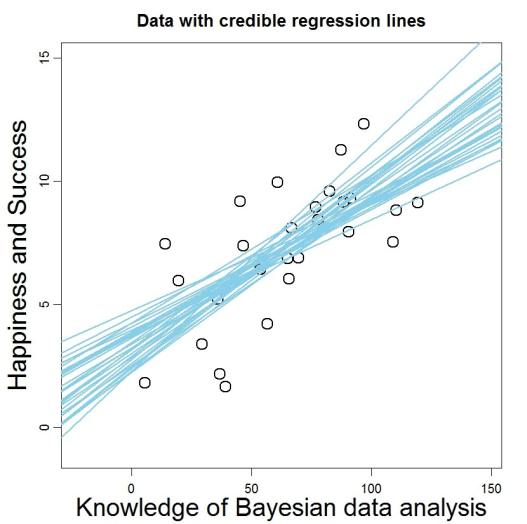
\includegraphics[width=0.6\textwidth]{images/happiness.png} \\
Credit: John Kruschke
\end{center}

\end{frame}


\begin{frame}
\frametitle{Plan}
\begin{itemize}
\item We will now look at two examples of Bayesian parameter estimation,
one of which also involves a {\bf prediction}.\pause
\item In both cases, we'll get the likelihood by defining the
{\bf sampling distribution} first.\pause
\item We will introduce a different ``non-informative'' prior distribution
that isn't uniform.
\end{itemize}

\end{frame}


\begin{frame}
\frametitle{Reminder of Bayes' Rule for Parameter Estimation}

\begin{align}
p(\theta \given x) &= \frac{p(\theta)p(x \given \theta)}{p(x)} \\
p(\theta \given x) &\propto p(\theta)p(x \given \theta) \\
\texttt{posterior} &\propto \texttt{prior} \times \texttt{likelihood}
\end{align}
(notation: $\theta$=parameter, $x$=data)

\end{frame}



\begin{frame}
\frametitle{Taxi Problem}

    \begin{columns} % Create two columns
        \column{0.5\textwidth} % Left column (50% width)

        \begin{itemize}
        \item You fall asleep in a foreign city.
        \item When you wake up in the morning, you see a taxi drive by,
              which says {\bf This is taxi number 42}.
        \item How many taxis are in the city?
        \end{itemize}

        \column{0.5\textwidth} % Right column (50% width)
        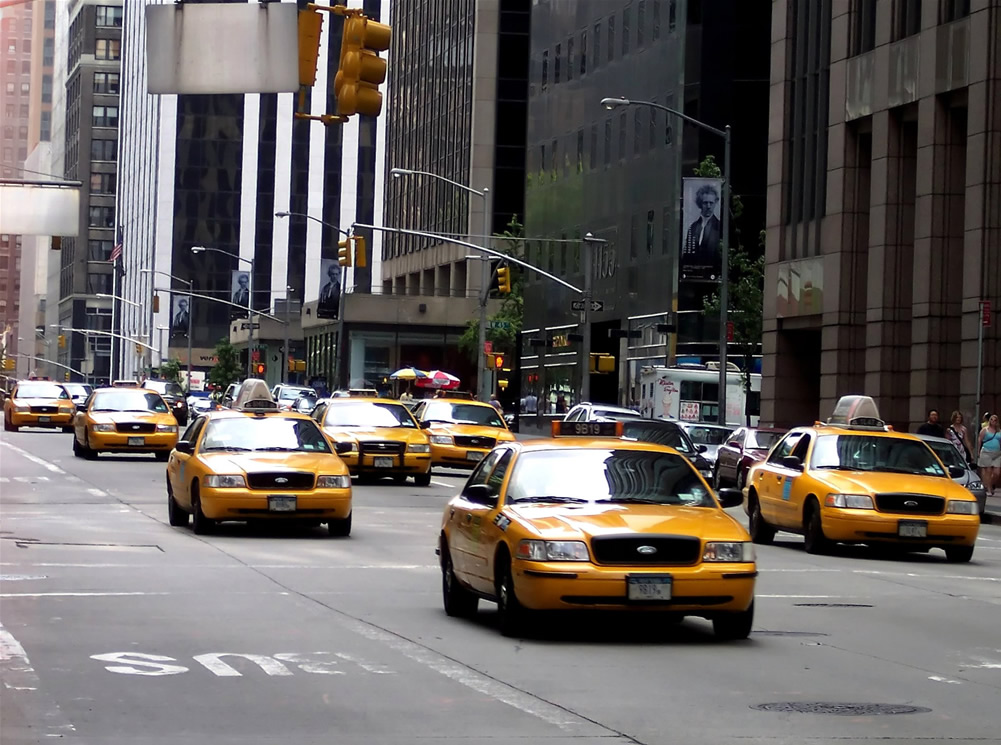
\includegraphics[width=0.95\linewidth]{images/taxis.jpg}
       
         (public domain image)
     \end{columns}

\end{frame}

\begin{frame}
\frametitle{The Parameter and the Data}

\begin{itemize}
\item The unknown parameter, $N$, is the number of taxis in the city.\pause
\item The data, $x$, is the number observed on the taxi that drove past.
\end{itemize}
\pause
Bayes' rule for this circumstance:

\begin{align}
p(N \given x) \propto p(N)p(x \given N)
\end{align}
We have to choose the prior $p(N)$ and the likelihood $p(x \given N)$.

\end{frame}


\begin{frame}
\frametitle{Bayes' Box with Uniform Prior}
Let's assume $N \leq 100$ and keep our uniform prior for now.

\centering
{\footnotesize
\begin{tabular}{|c|c|c|c|c|}
\hline
Parameter & Prior & Likelihood & Prior $\times$ Likelihood & Posterior \\
$N$  & $p(N)$ & $p(x \given N)$ & $p(N)p(x\given N)$ & $p(N\given x)$ \\
\hline
1 & 0.01 & & & \\
2 & 0.01  &  & & \\
... &... &... & ...&... \\
41 & 0.01 &  & & \\
42 & 0.01  &  & & \\
43 & 0.01 & & & \\
... &... &... & ...&... \\
99 & 0.01 & & & \\
100   & 0.01 & & & \\
\hline
Total & 1 & & & 1 \\
\hline
\end{tabular}
}

\end{frame}

\begin{frame}
\frametitle{Likelihoods: Direct Reasoning}

\begin{itemize}
\item If $N=1$, with what probability would we observe $x=42$? \pause
\item If $N=41$, with what probability would we observe $x=42$? \pause
\item If $N=42$, with what probability would we observe $x=42$? \pause
\item If $N=100$, with what probability would we observe $x=42$?
\end{itemize}

\end{frame}


\begin{frame}
\frametitle{Likelihoods}

\centering
{\footnotesize
\begin{tabular}{|c|c|c|c|c|}
\hline
Parameter & Prior & Likelihood & Prior $\times$ Likelihood & Posterior \\
$N$  & $p(N)$ & $p(x \given N)$ & $p(N)p(x\given N)$ & $p(N\given x)$ \\
\hline
1 & 0.01 & 0 & & \\
2 & 0.01  & 0  & & \\
... &... &... & ...&... \\
41 & 0.01 & 0 & & \\
42 & 0.01  & 1/42 & & \\
43 & 0.01 & 1/43 & & \\
... &... &... & ...&... \\
99 & 0.01 & 1/99 & & \\
100   & 0.01 & 1/100 & & \\
\hline
Total & 1 & & & 1 \\
\hline
\end{tabular}
}

\end{frame}


\begin{frame}
\frametitle{Likelihoods: from Sampling Distribution}
Imagine we did not know $x$ yet, but we did know $N$, the parameter.
We can assign a probability distribution for $x$ given $N$.
This would be a discrete uniform distribution, and we can write
\begin{align}
x \given N &\sim \textnormal{Uniform}(1, 2, ..., N).
\end{align}\pause

The formula for this probability distribution is
\begin{align}
p(x \given N) &= \left\{
                    \begin{array}{lr}
                    \frac{1}{N}, & x \in \{1, 2, ..., N\} \\
                    0          , & \textnormal{otherwise}.
                    \end{array}
                 \right.
\end{align}
\end{frame}

\begin{frame}
\frametitle{Likelihoods: from Sampling Distribution}
If we take the formula and interpret it as a function of $N$
with $x$ fixed at 42, it reads
\begin{align}
p(x \given N) &= \left\{
                    \begin{array}{lr}
                    \frac{1}{N}, & 42 \in \{1, 2, ..., N\} \\
                    0          , & \textnormal{otherwise}.
                    \end{array}
                 \right.
\end{align}
which is exactly the rule we `guessed' earlier.


\end{frame}

\begin{frame}
\frametitle{Likelihoods: from Sampling Distribution}
In general, we can think of data as being `drawn from'
some distribution\footnote{Philosophically I object, but it is a useful
starting point.}
with unknown parameter $\theta$, written as $p(x \given \theta)$.
This will be a formula involving both $x$ and $\theta$.
\pause

When $x$ is known value (plugged in) but $\theta$ isn't, $p(x \given \theta)$
is now a function of $\theta$ only --- the likelihood function.
You may have seen this in STATS 210 or other courses. If not, this is a
reasonable first place to learn about it.

\end{frame}


\begin{frame}
\frametitle{Likelihoods: from Sampling Distribution}
Since sampling distributions are conditional on $\theta$ but not on the
data $x$, they are kind of a prior but for the data instead of the parameter.

\end{frame}


\end{document}

